\documentclass[12pt, a4paper]{article}

% PACKAGES
\usepackage[margin=1in]{geometry}
\usepackage{amsmath}
\usepackage{graphicx}
\usepackage{siunitx}
\usepackage{tikz}
\usepackage[colorlinks=true, urlcolor=blue, linkcolor=black]{hyperref}
\usepackage{xcolor}
\usepackage{enumitem}

% TIKZ LIBRARIES
\usetikzlibrary{decorations.pathmorphing, patterns, arrows.meta, positioning}

% DOCUMENT INFO
\title{Advanced Problems on Photons and Quantum Physics}
\author{}
\date{\today}

% BEGIN DOCUMENT
\begin{document}

\maketitle
\tableofcontents
\newpage

\section{New Practice Problems}

\subsection{Problem 1: The Photoelectric Effect on an Unknown Metal}
\begin{quote}
    Light with a wavelength of \SI{250}{\nano\meter} is incident on an unknown metal plate. The emitted photoelectrons are found to have a maximum kinetic energy of \SI{2.95}{\electronvolt}.
\end{quote}

\subsubsection*{(a) What is the work function of the metal in electron-volts (eV)?}
\textbf{Explanation:} We can find the energy of the incident photons using the equation $E = hc/\lambda$. Then, using Einstein's photoelectric equation ($K_{max} = E_{photon} - \phi$), we can rearrange it to solve for the work function, $\phi$.

\textbf{Solution:}
\begin{enumerate}[label*=\arabic*.]
    \item \textbf{Calculate the energy of the incident photons ($E_{\text{photon}}$):}\\
    First, it's often easier to work in electron-volts. A useful constant is $hc \approx \SI{1240}{\electronvolt\nano\meter}$.
    \[ E_{\text{photon}} = \frac{hc}{\lambda} = \frac{\SI{1240}{\electronvolt\nano\meter}}{\SI{250}{\nano\meter}} = \SI{4.96}{\electronvolt} \]

    \item \textbf{Calculate the work function ($\phi$):}\\
    Rearranging Einstein's photoelectric equation:
    \begin{align*}
        \phi &= E_{\text{photon}} - K_{\text{max}} \\
             &= \SI{4.96}{\electronvolt} - \SI{2.95}{\electronvolt} \\
             &= \SI{2.01}{\electronvolt}
    \end{align*}
\end{enumerate}
\textbf{Final Answer:} The work function of the metal is \textbf{\SI{2.01}{\electronvolt}}.

\subsubsection*{(b) What is the cutoff wavelength ($\lambda_c$) for this metal?}
\textbf{Explanation:} The cutoff wavelength is the longest wavelength of light that can cause photoemission. At this wavelength, the photon has just enough energy to overcome the work function ($\phi$), so the kinetic energy of the emitted electron is zero. The energy of the photon is therefore equal to the work function: $\phi = hc/\lambda_c$.

\textbf{Solution:}
\begin{enumerate}[label*=\arabic*.]
    \item \textbf{Calculate the cutoff wavelength ($\lambda_c$):}\\
    Rearranging the energy equation:
    \[ \lambda_c = \frac{hc}{\phi} = \frac{\SI{1240}{\electronvolt\nano\meter}}{\SI{2.01}{\electronvolt}} \approx \SI{617}{\nano\meter} \]
\end{enumerate}
\textbf{Final Answer:} The cutoff wavelength is \textbf{\SI{617}{\nano\meter}}.

\hrulefill
\subsection{Problem 2: Solar Sail Propulsion}
\begin{quote}
    A small interplanetary probe has a mass of \SI{500}{\kilo\gram} and is propelled by a perfectly reflecting solar sail with an area of \SI{400}{\meter\squared}. The probe is currently at a distance from the Sun where the intensity of solar radiation is \SI{1360}{\watt\per\meter\squared}.
\end{quote}
\begin{figure}[h!]
    \centering
    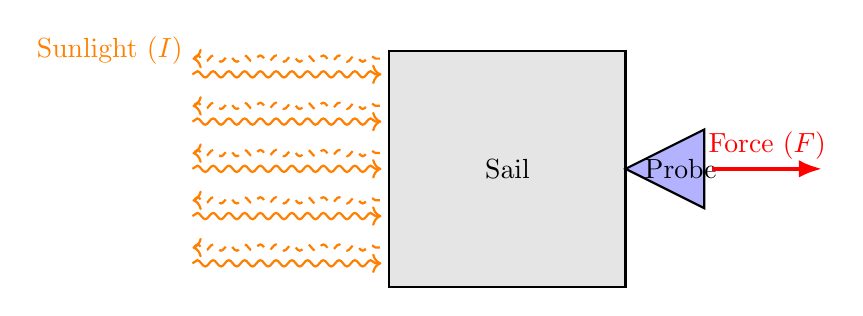
\begin{tikzpicture}[scale=1.0, transform shape]
        % Solar Sail
        \draw[fill=gray!20, thick] (-1.5, -1.5) rectangle (1.5, 1.5);
        \node at (0, 0) {Sail};

        % Probe Body
        \draw[fill=blue!30, thick] (1.5, 0) -- (2.5, 0.5) -- (2.5, -0.5) -- cycle;
        \node at (2.2, 0) {Probe};
        
        % Incident Photons (Sunlight)
        \foreach \y in {-1.2, -0.6, 0, 0.6, 1.2} {
            \draw[->, thick, orange, decorate, decoration={snake, amplitude=0.4mm, segment length=2mm}] (-4, \y) -- (-1.6, \y);
        }
        \node[left, orange] at (-4, 1.5) {Sunlight ($I$)};

        % Reflected Photons
        \foreach \y in {-1.2, -0.6, 0, 0.6, 1.2} {
            \draw[<-, thick, orange, dashed, decorate, decoration={snake, amplitude=0.4mm, segment length=2mm}] (-4, \y+0.2) -- (-1.6, \y+0.2);
        }
        
        % Force Vector
        \draw[->, -{Latex[length=3mm]}, ultra thick, red] (2.6, 0) -- (4, 0);
        \node[above, red] at (3.3, 0) {Force ($F$)};
    \end{tikzpicture}
    \caption{Diagram of a solar sail being propelled by radiation pressure.}
    \label{fig:solarsail}
\end{figure}

\subsubsection*{(a) What is the force exerted on the solar sail?}
\textbf{Explanation:} Since the sail is perfectly reflecting, the radiation pressure it experiences is given by $P_{\text{rad}} = 2I/c$. The total force is this pressure multiplied by the area of the sail, $F = P_{\text{rad}} \cdot A$.

\textbf{Solution:}
\begin{enumerate}[label*=\arabic*.]
    \item \textbf{Calculate the radiation pressure ($P_{\text{rad}}$):}
    \[ P_{\text{rad}} = \frac{2I}{c} = \frac{2(\SI{1360}{\watt\per\meter\squared})}{\SI{3.00e8}{\meter\per\second}} \approx \SI{9.07e-6}{\newton\per\meter\squared} \]
    
    \item \textbf{Calculate the force ($F$):}
    \[ F = P_{\text{rad}} \cdot A = (\SI{9.07e-6}{\newton\per\meter\squared})(\SI{400}{\meter\squared}) \approx \SI{3.63e-3}{\newton} \]
\end{enumerate}
\textbf{Final Answer:} The force on the sail is \textbf{\SI{3.63e-3}{\newton}}.

\subsubsection*{(b) What is the initial acceleration of the probe?}
\textbf{Explanation:} Using Newton's Second Law of Motion ($F=ma$), we can find the acceleration by dividing the force calculated in part (a) by the mass of the probe.

\textbf{Solution:}
\[ a = \frac{F}{m} = \frac{\SI{3.63e-3}{\newton}}{\SI{500}{\kilo\gram}} \approx \SI{7.26e-6}{\meter\per\second\squared} \]
\textbf{Final Answer:} The probe's acceleration is \textbf{\SI{7.26e-6}{\meter\per\second\squared}}.

\hrulefill
\subsection{Problem 3: Excitation of Helium Ions}
\begin{quote}
    A stationary, singly-ionized helium atom ($He^+$) in its ground state ($n=1$) is struck by a photoelectron. The energy levels of a hydrogen-like ion are given by $E_n = -Z^2 \frac{\SI{13.6}{\electronvolt}}{n^2}$, where $Z$ is the atomic number.
\end{quote}

\subsubsection*{(a) If the photoelectron has a kinetic energy of \SI{49.2}{\electronvolt}, what is the highest energy level ($n$) that the $He^+$ ion can be excited to?}
\textbf{Explanation:} First, we calculate the energies of the stationary states of the $He^+$ ion ($Z=2$). Then, we find the energy required to excite the ion from the ground state to higher levels. The electron can only cause an excitation if its kinetic energy is greater than or equal to the required excitation energy.

\textbf{Solution:}
\begin{enumerate}[label*=\arabic*.]
    \item \textbf{Calculate the ground state energy ($E_1$) of $He^+$ ($Z=2$):}
    \[ E_1 = -2^2 \frac{\SI{13.6}{\electronvolt}}{1^2} = \SI{-54.4}{\electronvolt} \]

    \item \textbf{Calculate the energies of the excited states ($E_n$):}
    \begin{itemize}
        \item $n=2: E_2 = -4 \cdot \frac{\SI{13.6}{4}} = \SI{-13.6}{\electronvolt}$
        \item $n=3: E_3 = -4 \cdot \frac{\SI{13.6}{9}} \approx \SI{-6.04}{\electronvolt}$
        \item $n=4: E_4 = -4 \cdot \frac{\SI{13.6}{16}} = \SI{-3.4}{\electronvolt}$
    \end{itemize}

    \item \textbf{Calculate the excitation energies ($\Delta E$) from the ground state:}
    \begin{itemize}
        \item To $n=2: \Delta E_{1 \to 2} = E_2 - E_1 = -13.6 - (-54.4) = \SI{40.8}{\electronvolt}$
        \item To $n=3: \Delta E_{1 \to 3} = E_3 - E_1 = -6.04 - (-54.4) = \SI{48.36}{\electronvolt}$
        \item To $n=4: \Delta E_{1 \to 4} = E_4 - E_1 = -3.4 - (-54.4) = \SI{51.0}{\electronvolt}$
    \end{itemize}

    \item \textbf{Compare the electron's energy to the excitation energies:}\\
    The photoelectron's energy is $K = \SI{49.2}{\electronvolt}$.
    \begin{itemize}
        \item $K > \Delta E_{1 \to 2}$ (\SI{40.8}{eV}) $\implies$ Excitation to $n=2$ is possible.
        \item $K > \Delta E_{1 \to 3}$ (\SI{48.36}{eV}) $\implies$ Excitation to $n=3$ is possible.
        \item $K < \Delta E_{1 \to 4}$ (\SI{51.0}{eV}) $\implies$ Excitation to $n=4$ is not possible.
    \end{itemize}
\end{enumerate}
\textbf{Final Answer:} The highest energy level the ion can be excited to is \textbf{$n=3$}.

\subsubsection*{(b) What are the possible wavelengths of photons emitted as the excited ion de-excites?}
\textbf{Explanation:} After being excited to the $n=3$ level, the ion will de-excite. It can do this in two ways: a direct transition ($n=3 \to n=1$), or a cascade transition ($n=3 \to n=2$ then $n=2 \to n=1$). Each transition emits a photon whose energy equals the energy difference between the levels. The wavelength is found using $\lambda = hc/E$.

\begin{figure}[h!]
    \centering
    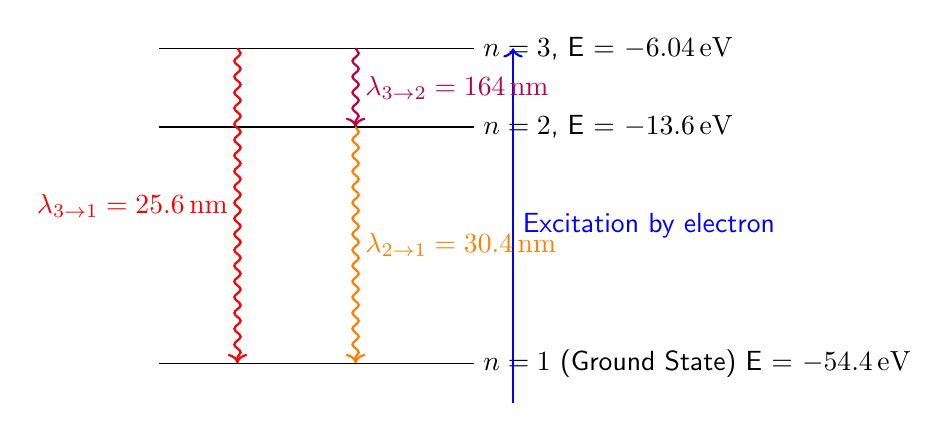
\begin{tikzpicture}[font=\sffamily]
        % Energy Levels
        \draw (0,0) -- (4,0) node[right] {$n=1$ (Ground State) E = \SI{-54.4}{\electronvolt}};
        \draw (0,3) -- (4,3) node[right] {$n=2$, E = \SI{-13.6}{\electronvolt}};
        \draw (0,4) -- (4,4) node[right] {$n=3$, E = \SI{-6.04}{\electronvolt}};
        
        % Excitation Arrow
        \draw[->, thick, blue] (4.5, -0.5) -- (4.5, 4);
        \node[right, blue] at (4.5, 1.75) {Excitation by electron};

        % De-excitation arrows and labels
        % 3 -> 1 transition
        \draw[->, thick, red, decorate, decoration={snake, amplitude=0.4mm, segment length=2mm}] (1,4) -- (1,0);
        \node[left, red] at (1,2) {$\lambda_{3 \to 1} = \SI{25.6}{\nano\meter}$};
        
        % 3 -> 2 transition
        \draw[->, thick, purple, decorate, decoration={snake, amplitude=0.4mm, segment length=2mm}] (2.5,4) -- (2.5,3);
        \node[right, purple] at (2.5, 3.5) {$\lambda_{3 \to 2} = \SI{164}{\nano\meter}$};
        
        % 2 -> 1 transition
        \draw[->, thick, orange, decorate, decoration={snake, amplitude=0.4mm, segment length=2mm}] (2.5,3) -- (2.5,0);
        \node[right, orange] at (2.5, 1.5) {$\lambda_{2 \to 1} = \SI{30.4}{\nano\meter}$};
        
    \end{tikzpicture}
    \caption{Energy level diagram for $He^+$ showing possible de-excitation pathways from the $n=3$ state.}
    \label{fig:he_levels}
\end{figure}

\textbf{Solution:}
\begin{enumerate}[label*=\arabic*.]
    \item \textbf{Calculate the wavelengths for each possible transition using $\lambda = hc/E$:}\\
    \begin{itemize}
        \item \textbf{Transition $3 \to 1$}: $\Delta E = \SI{48.36}{\electronvolt}$
        \[ \lambda_{3 \to 1} = \frac{\SI{1240}{\electronvolt\cdot\nano\meter}}{\SI{48.36}{\electronvolt}} \approx \SI{25.6}{\nano\meter} \]
        
        \item \textbf{Transition $3 \to 2$}: $\Delta E = E_3 - E_2 = -6.04 - (-13.6) = \SI{7.56}{\electronvolt}$
        \[ \lambda_{3 \to 2} = \frac{\SI{1240}{\electronvolt\cdot\nano\meter}}{\SI{7.56}{\electronvolt}} \approx \SI{164}{\nano\meter} \]
        
        \item \textbf{Transition $2 \to 1$}: $\Delta E = \SI{40.8}{\electronvolt}$
        \[ \lambda_{2 \to 1} = \frac{\SI{1240}{\electronvolt\cdot\nano\meter}}{\SI{40.8}{\electronvolt}} \approx \SI{30.4}{\nano\meter} \]
    \end{itemize}
\end{enumerate}
\textbf{Final Answer:} The possible emitted wavelengths are approximately \textbf{\SI{25.6}{\nano\meter}}, \textbf{\SI{30.4}{\nano\meter}}, and \textbf{\SI{164}{\nano\meter}}.

\end{document}